\section{BrowseController Class Reference}
\label{classBrowseController}\index{BrowseController@{BrowseController}}
Inheritance diagram for BrowseController:\nopagebreak
\begin{figure}[H]
\begin{center}
\leavevmode
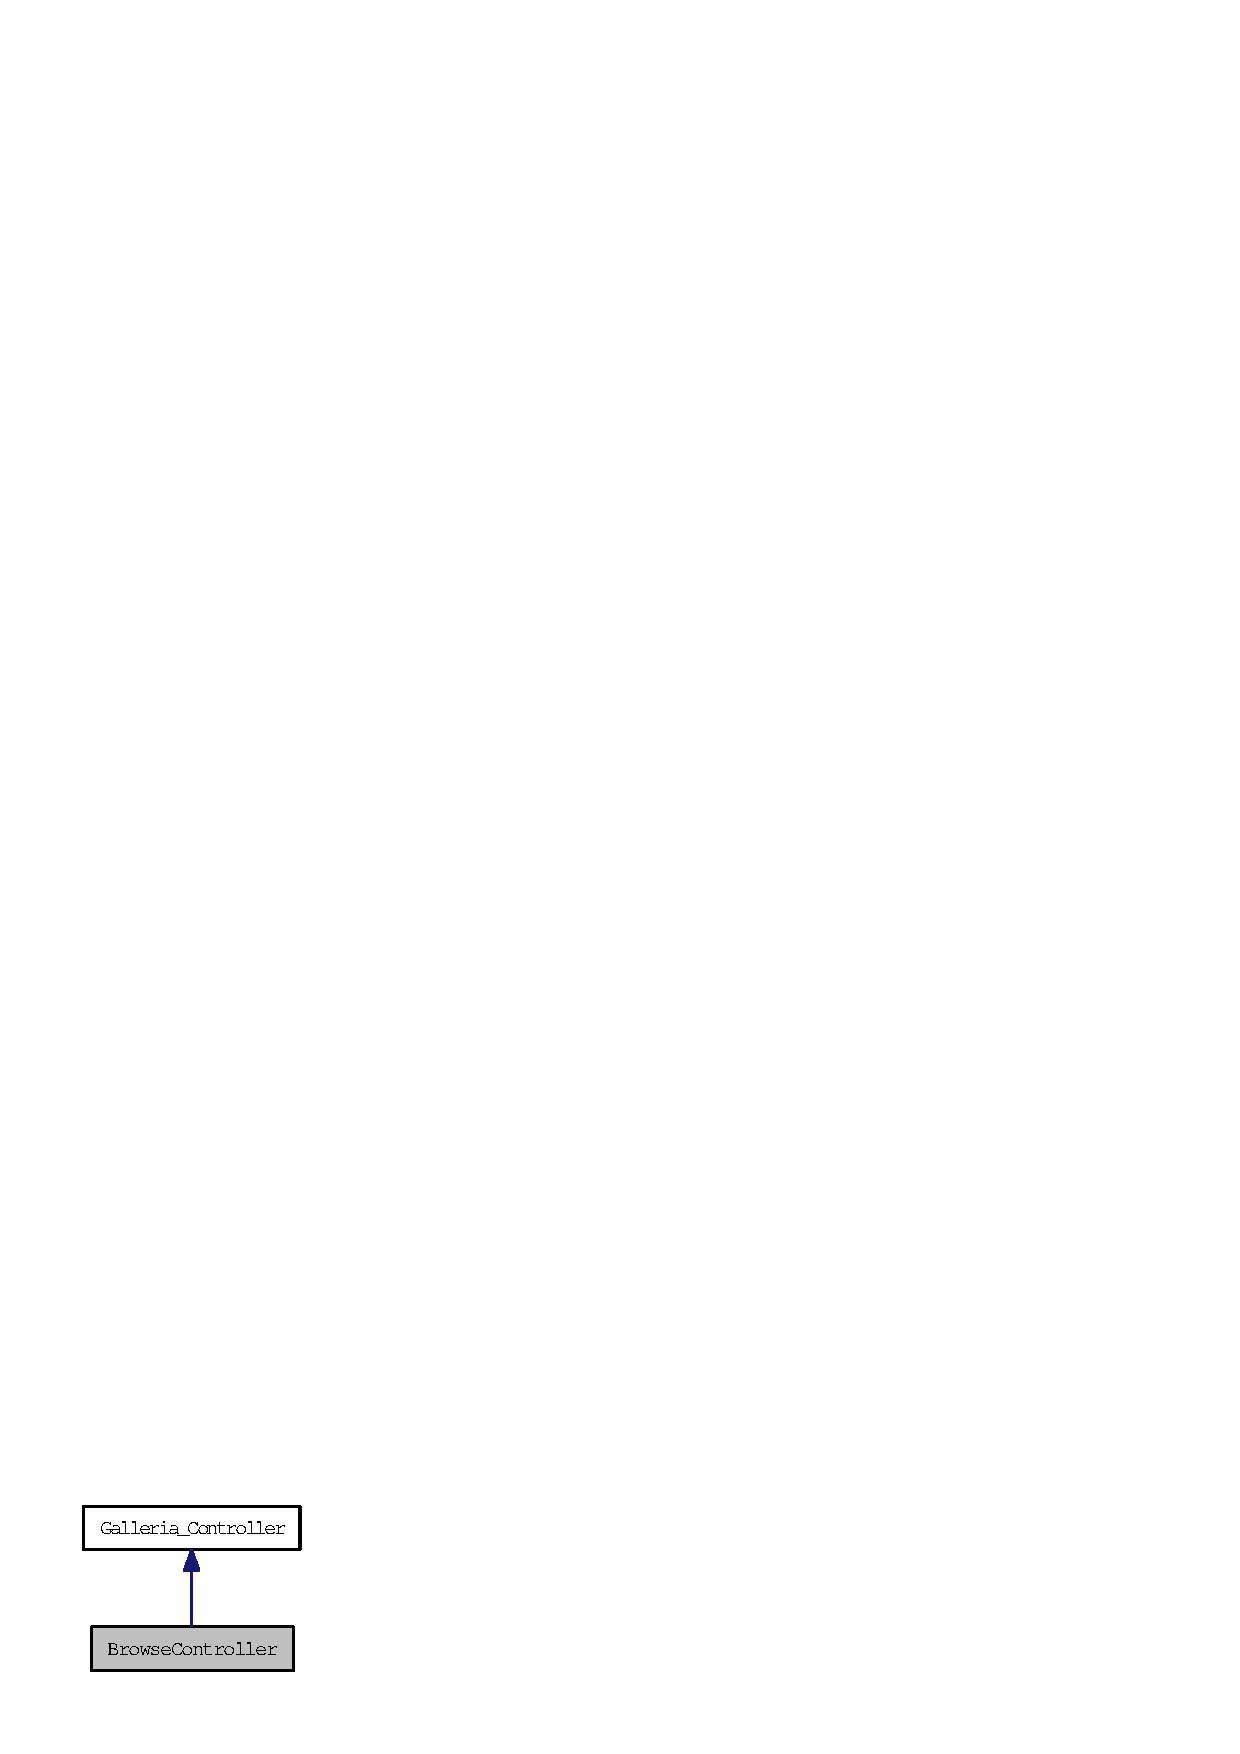
\includegraphics[width=74pt]{classBrowseController__inherit__graph}
\end{center}
\end{figure}
Collaboration diagram for BrowseController:\nopagebreak
\begin{figure}[H]
\begin{center}
\leavevmode
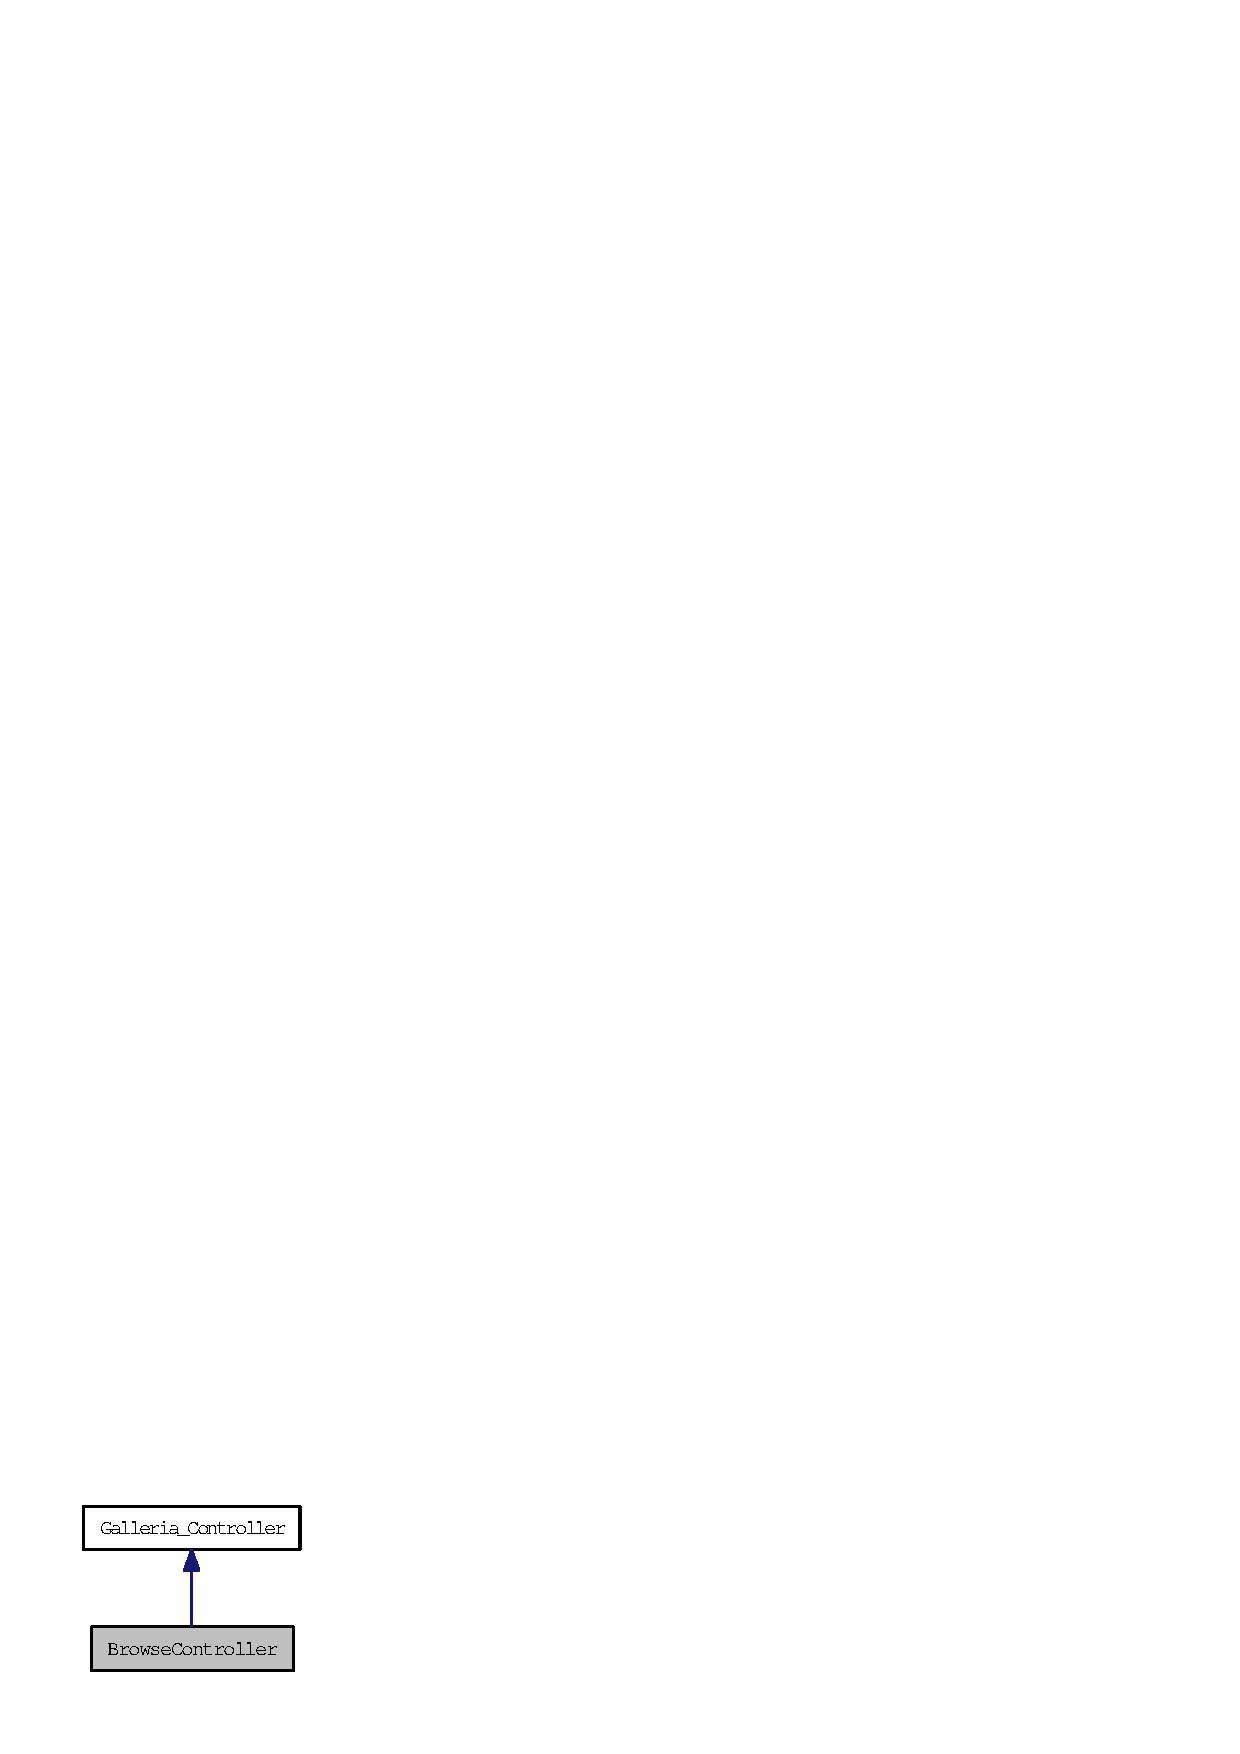
\includegraphics[width=74pt]{classBrowseController__coll__graph}
\end{center}
\end{figure}
\subsection*{Public Member Functions}
\begin{CompactItemize}
\item 
{\bf indexAction} ()
\end{CompactItemize}


\subsection{Detailed Description}


Definition at line 19 of file browsecontroller.php.

\subsection{Member Function Documentation}
\index{BrowseController@{BrowseController}!indexAction@{indexAction}}
\index{indexAction@{indexAction}!BrowseController@{BrowseController}}
\subsubsection{\setlength{\rightskip}{0pt plus 5cm}BrowseController.indexAction ()}\label{classBrowseController_c12a5cf382694a070e902cb5555d9726}


Index page.

Index page action. Sets up Browse index page.  public 

Definition at line 28 of file browsecontroller.php.

References Galleria\_\-Controller.\_\-getModel(), Galleria\_\-Element\_\-Category.create(), and Galleria\_\-Controller.getView().

Here is the call graph for this function:\nopagebreak
\begin{figure}[H]
\begin{center}
\leavevmode
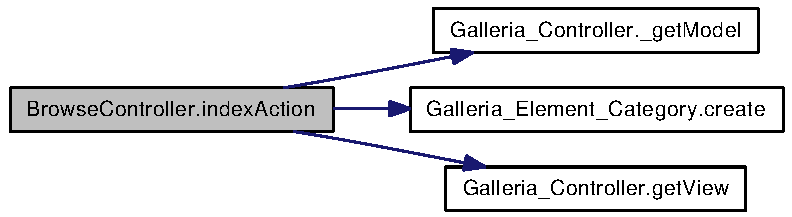
\includegraphics[width=208pt]{classBrowseController_c12a5cf382694a070e902cb5555d9726_cgraph}
\end{center}
\end{figure}


The documentation for this class was generated from the following file:\begin{CompactItemize}
\item 
/var/www/galleria/data/site/mvc/controller/{\bf browsecontroller.php}\end{CompactItemize}
